% This is an included file. See the master file for more information.
%

\section{Execution Model}
\index{Execution Model}
\label{sec:ExecutionModel}

An OCR program\index{OCR program} is best understood as a dynamically created,
directed acyclic graph
(DAG)\index{DAG}~\cite{TaSa11,Tasirlar11,Zuckerman:2011:UCP:2000417.2000424}.
The vertices in the graph are OCR objects that define a computation:
tasks\index{Task} which perform the actual computation and
events\index{Event} which are used to coordinate the
activity of other objects. The edges are dependences between objects
(i.e.\ a \emph{link}) which can represent data dependences (events with
an associated data block) or pure control dependences (events).

The tasks within the DAG represent the work carried out by an OCR
program. Edges impinging on a task define preconditions for the execution of
the task~\cite{SSWS13}. Tasks whose preconditions have been met are
\emph{runnable}\index{Runnable}. Outgoing edges define dependences and
triggers for later objects in the graph. OCR tasks are
\emph{non-blocking}\index{non-blocking}. This means that once all
preconditions on a task have been met, the task becomes runnable, and
when it begins to execute; the task will eventually run to completion
regardless of the behavior of any other OCR objects.

OCR programs can either run alone or be encompassed in other programs
in a library manner. In the following description, ``OCR program'' refers
to either the entire OCR program if it is running alone or the OCR
portion of the program if running library mode.

The OCR program logically starts as a single task, dynamically builds the
DAG corresponding to the executing program, and completes when the
\code{ocrShutdown()} or \code{ocrAbort()} function is called.
This rather simple model can handle a wide range of
design patterns including branch and bound, data flow, and divide and
conquer.
%
%Vivek wanted to add a long discusssion of how you can use to represent
% SPMD algorithms as well. Once again, given the short time to address this,
% I opted to leave it out. This is a specfication not a programmers reference guide. But
% he rasied many good points that we need to develop and docuent somewhere
%
With both data and tasks conceptually decoupled from their realization
on a computer system, OCR has the flexibility to relocate tasks and data
to respond to failures in the system, achieve a better balance of load
among the processing elements of the computer, or to optimize memory
and energy consumption~\cite{GZCS10,Guo10,CTBCCGYS13,SbBS14}.

We will define the execution model in OCR by starting with a model of
the OCR platform. We will then describe the fundamental objects used
to define OCR. Finally, we will describe the details of how an OCR
program executes.


\begin{figure*}
\centering
 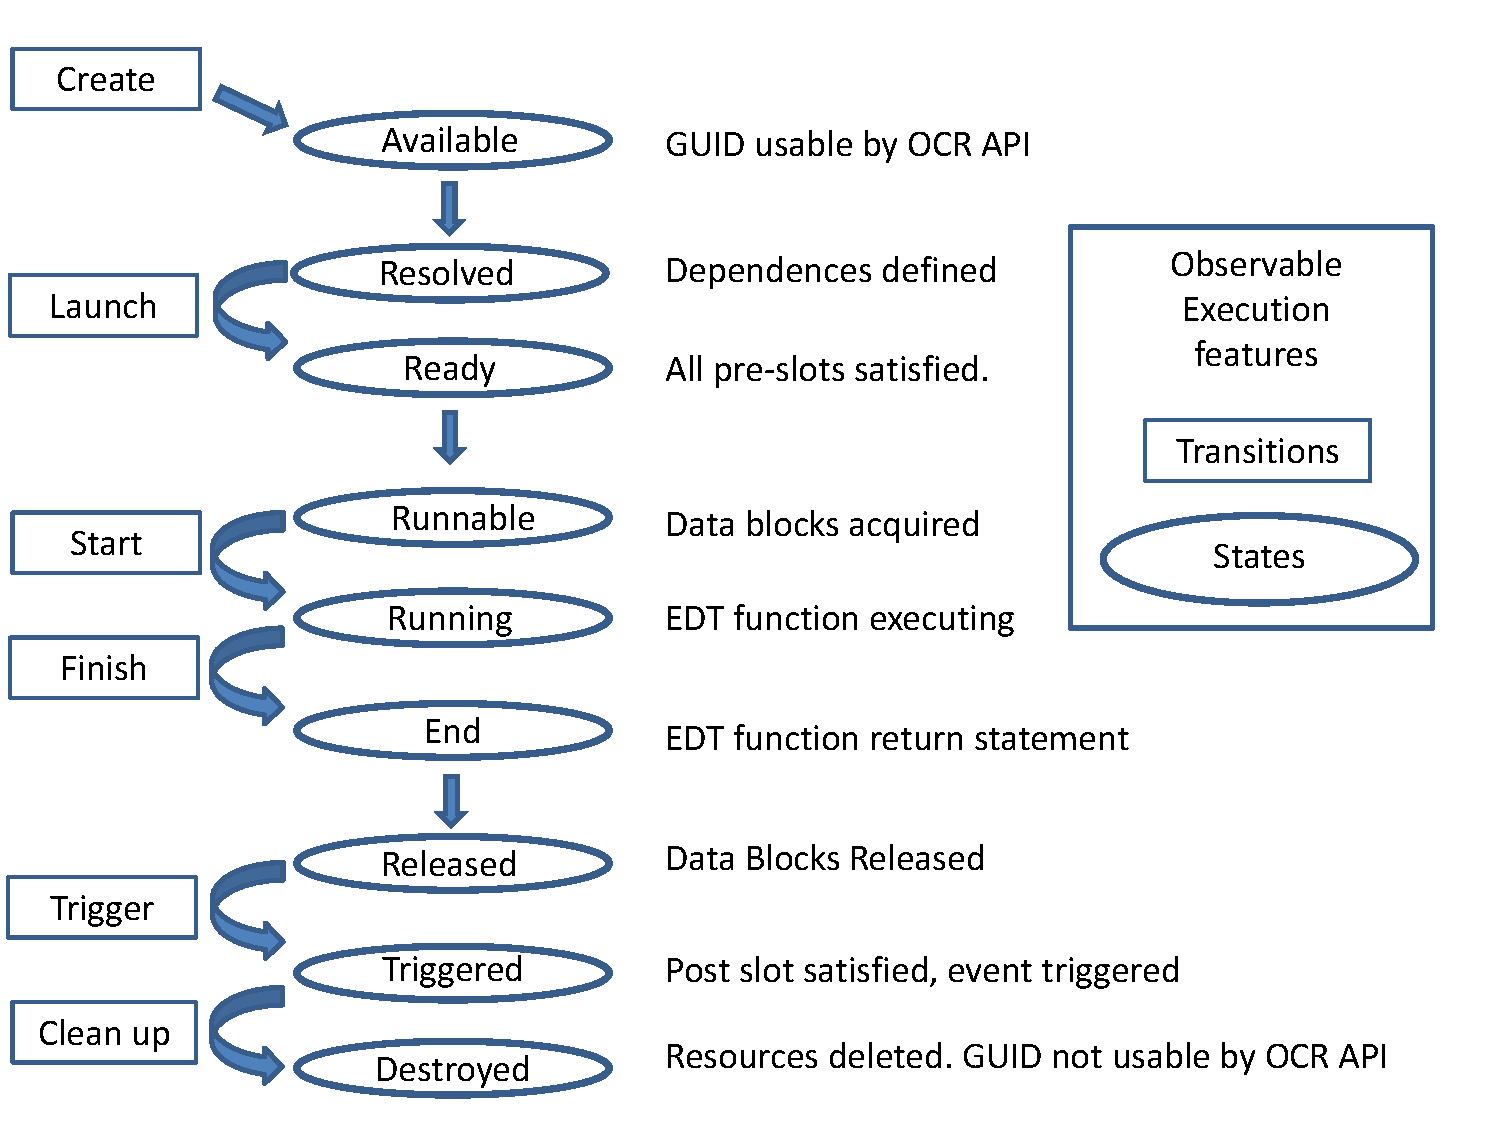
\includegraphics[width=0.9\textwidth]{EDT_exec}
\caption{Obseevable exectuion features.}
\label{fig:EDTexec}
\end{figure*}
%
%\FigRef{fig:EDT_exec.pdf}
%
%
%\ScaledDiagram{EDT execution: observable states and transitions}%
%{fig:EDT_exec}%
%{EDT_exec}
%{0.5}

\subsection{OCR Platform}
\index{OCR Platform}
\label{sec:OCRPlatform}

An OCR program executes on an abstract machine called the \emph{OCR
Platform}.  The OCR platform is a resource that can carry out
computations. It consists of:
\begin{itemize}
\item A collection of network connected nodes where any two nodes can
communicate with each other.
\item Each node consists of one or more processing elements each of
which has its own private memory\footnote{By ``private'' we mean a
memory region that is not accessible to other processing
elements.}.
\item A globally accessible shared namespace of OCR objects each
denoted by a globally unique ID (GUID).
\end{itemize}
OCR is designed to be portable and scalable, hence, the OCR Platform
places minimal constraints on the physical hardware.

As dependences are met for the tasks in an OCR program's DAG, the
tasks become \emph{runnable}. These tasks and any resources required
to support their execution are then submitted to
\emph{workers}\index{Worker}~\cite{GBRS09} which execute the tasks on
the processing elements within the OCR platform. The workers and the
data-structures used to store tasks waiting to execute
(i.e.\ work-pools) are a low level implementation detail not defined by
the OCR specification. When reasoning about locality and load
balancing, programmers may need to explicitly reason about the
behavior of the workers~\cite{Chatterjee13}, but they do not hold
persistent state visible to an OCR program and are logically opaque to
OCR constructs.
%
% vivek added ...
%Tuning annotations for locality can be specified in OCR in the form of preferred affinities (co-location)
% among EDTs and/or data blocks.
%
% TGM responds ... I didn't see this anywhere in the current API. Did I miss something?  If they aren't there
% we can't put them in the spec. If they are there, we need to talk about this and figure out how
% to add this to the spec.
% REC: They are still being defined and are not solidly fixed
% yet. Zoran, Sanjay and Rob are discussing them.

\subsection{OCR objects}
\index{OCR object}
\label{sec:OCRobjects}

An OCR object is a reference counted entity managed by OCR. Every OCR
object has a globally unique ID (GUID) that is used to identify the
object. Objects have two well defined states.
\begin{enumerate}
\item \emph{Created}: Resources associated with an object and its GUID
have been created.
\item \emph{Destroyed}: An object that is destroyed is marked for
destruction when the destruction command executes. A destroyed object
and any resources associated with the destroyed object are no longer
defined. The object is not actually destroyed and the associated
resources are not freed until the reference count is zero\footnote{As
an optimization, the runtime may choose to reuse of the same physical
object for different logical objects~\cite{USBCSS12,SbKS12}.}.
%
%  Vivek suggest we call this "Dead" instead of "destroyed".  He provided new text in his feedback to
% address this. I wouild have put his text here, but I can't cut and paste from his document. But
% if we all agree, we should look at his feedback document and add this later.
\end{enumerate}
Furthermore, for OCR data blocks, we have two additional states:
\begin{enumerate}
\item \emph{Acquired}: the data associated with the data block has
become accessible to the acquiring OCR object thereby incrementing the
acquired objects reference count.
\item \emph{Released}: The object is no longer accessible by the OCR
object that had earlier acquired it. The reference count on the
released object is decremented.
\end{enumerate}

An OCR program is defined in terms of three fundamental objects.
\begin{description}
\item[Event Driven Tasks (EDT)] A non-blocking unit of work in an OCR
program.
\item[Data blocks (DB)] A contiguous block of memory managed by the
OCR runtime accessible to any OCR objects to which it is linked.
\item[Events] An object to manage dependences between OCR objects and
to define ordering relationships (synchronization) between them.
\end{description}

In addition to these fundamental objects, OCR defines a number of
associated objects that simplify OCR programming or support specific
desired behaviors of the fundamental objects.
\begin{description}
\item [EDT Template] An OCR object used to manage the resources
required to create an EDT.
\item [Affinity container] An OCR object used to influence the
placement of EDTs in an executing program.
\end{description}

An OCR program defines a graph with the three fundamental OCR objects
(EDTs, DBs and Events) as the nodes of the graphs and edges are
\emph{links}\index{Link} between objects. A link defines a dependence
between OCR objects. The links are defined in terms of
\emph{slots}\index{Slot} on the OCR object. A slot defines an end
point for a dependence for an OCR object.

Event, data blocks and EDTs each have a single \emph{post
slot}\index{post-slot}.  used to communicate the state of an OCR
object to other OCR objects. For example, if an EDT wanted to let
another EDT know that it had finished its assigned work, it could do
so by signaling over its post-slot that it is \emph{satisfied} or
equivalently, that the post-slot is \emph{triggered}. The rules
defining when a post slot triggers, the so-called \emph{post-slot
trigger rule}\index{post-slot trigger rule} depends on the type of OCR
object and is discussed in Section~\ref{sec:triggerrule}.

Some OCR objects (such as EDTs) can also have an optional set of
\emph{pre-slots}\index{pre-slot}. A pre-slot defines an incoming
dependence or a pre-condition for execution by an EDT. The post-slot
of one EDT, for example, can be connected to the pre-slot of another
EDT thereby establishing a control dependence\index{control
dependence} between the EDTs. Likewise,
the post-slot of a data block can be connected to the pre-slot of an EDT
to establish an immediately satsified data dependence.

Slots are used along with data block objects to define data
dependences\index{data dependence} between OCR objects. For example,
for producer consumer relationships\index{producer consumer
relationships} the post slot of the producer EDT can be connected to
the pre-slot of the consumer EDT. When the producer finishes its work
and updates the data block it wishes to share, it associates that data
block with the post-slot and signals its ``satisfied'' state to the
consumer who can then safely begin working with the data block from
the producer.

Refer to Section~\ref{sec:Glossary} for a definition of the states of
a Slot. All slots are initially in the \code{unconnected} state. Data
block post slots are immediately \code{satisfied} as soon as they are
connected.
\subsubsection{EDTs}
\index{EDT}
\label{sec:EDT}

A task defines the basic unit of work within a programming model. As
mentioned earlier, a task is a non-blocking unit of work. Once all
pre-conditions on the OCR task have been met, it becomes
runnable\index{Runnable} or ``available to execute'' and once it
begins execution it executes without waiting on any other OCR
objects. In OCR, we package a task into an Event Driven
Task\index{Event Driven Task} or an EDT\index{EDT}.

The EDT is created as an instance of an \emph{EDT template}\index{EDT
template}. This template stores metadata about EDTs created from the
template, optionally defines the number of dependences and parameters
used when creating an instance of an EDT, and is a container for the
function that will be executed by an EDT. This function is called the
\emph{EDT function}\index{EDT function}.

The OCR API defines the function prototype and return values expected
by an EDT function. These include:
\begin{itemize}
\item The parameters of the EDT function which are copied by value
when the EDT is created.
\item Dynamic dependences expressed through a dependence array that is
formed at runtime from explicit user-specified dependences.
\item An optional GUID of a OCR object holding data (a \emph{data
block}) that will be used to satisfy the EDT’s post slot. This is the
return value of the function.
\end{itemize}
When \code{ocrEdtCreate()} is used to create an EDT, it returns one or
two GUIDs: the first (always returned) is the GUID for the EDT itself;
the second (returned only on programmer request) is the GUID of the
event implied by the post slot of the EDT\footnote{It is important to
  note that although, semantically, an EDT can be the source of a
  dependence, when adding a dependence, the programmer must use the
  GUID of the associated event as the source.}
When the OCR function returns a data block, the GUID of
that data block is used to satisfy the implied event.

Using a post-slot in a link to another object is just one method to
trigger other OCR objects. OCR includes the \code{ocrEventSatisfy()}
API to trigger other OCR objects through explicitly created dependence
links.

OCR defines one special type of EDT; the \emph{finish
EDT}\index{Finish EDT}. An EDT always executes asynchronously and
without blocking once all of its pre-conditions have been met. A
finish EDT, however, will not trigger its post-slot until all EDTs
launched within its scope (i.e.\ its child EDTs and EDTs created
within its child EDTs) have completed.  The finish EDT still executes
asynchronously and without blocking. The implied event associated with
the post slot of a finish EDT is a \emph{latch event}, i.e.\ it is
connected to the post-slots of all EDTs created within its scope and
does not trigger until they have all finished.

\subsubsection{Events}
\index{Event}
\label{sec:Event}

An event is an OCR object used to coordinate the activity of other OCR
objects. As with any OCR object, events have a single
post-slot. Events may also have one or more pre-slots; the actual
number of which is determined by the type of event.

The post-slot of an event can be connected to multiple OCR objects by
connecting the single post-slot to the pre-slots of other OCR objects.
When the conditions are met indicating that the event should trigger
(according to the \emph{trigger rule}\index{trigger rule}), the event
sets its post-slot to \emph{satisfied} therefore establishing an
ordering relationship between the event and the OCR objects linked to
the event. Events therefore play a key role in establishing the
patterns of synchronization required by a parallel
algorithm~\cite{ImSa14-2}.

When an event is satisfied, it can optionally attach a data block to
the post slot. Hence, events not only provide synchronization
(control dependences) but they are also the mechanism OCR uses to
establish data flow dependences. In other words, a classic data flow
algorithm defines tasks as waiting until data is ``ready''. In OCR
this concept is implemented through events with attached data blocks.

Given the diversity of parallel algorithms, OCR has defined several
types of events:
\begin{enumerate}
\item \emph{Once event}\index{Event, Once}: The event is automatically
destroyed on satisfaction. Any object that has the Once event as a
pre-condition must already have been created and linked by the time
the Once event is satisfied.

\item \emph{Idempotent event}\index{Event, Idempotent}: The event
exists until explicitly destroyed by a call to
\code{ocrEventDestroy()}. It is satisfied once and subsequent attempts
to satisfy (i.e.\ trigger) the event are ignored.

\item \emph{Sticky event}\index{Event, Sticky}: The event exists until
explicitly destroyed with a call to \code{ocrEventDestroy()}. It is
satisfied once and subsequent attempts to satisfy (i.e.\ trigger) the
event result in an error code being returned when trying to satisfy
the event.
%
%  Vivek writes:  Need to state the meaning of an error in OCR. Does it result in program
% termination, or some sort of error code (since there is no support for exceptions in C),
% or is it simply undefined?
%
%  TGM respondes ... yes, I am in violent agreement with Vivek. I just don't know
% how to do this right now in fits in with the overall design of OCR. This shojld be
% a major discussion point following the apps workshop
% REC: I added a small note saying it is an error code
%
\item \emph{Latch event}\index{Event, Latch}: The latch event has two
pre-slots and triggers when the conditions defined by the latch
trigger rule are met. The event is automatically destroyed once it
triggers; in this regard, it is similar to a \emph{once event}.
\end{enumerate}
Events have one pre-slot except for latch-events which have two pre-slots.

\subsection{Trigger rule}
\label{sec:triggerrule}
Events ``trigger'' when the appropriate \emph{trigger
rule}\index{trigger rule} is met. The default trigger rule for events
is when the link on their pre-slot is satisfied, the event triggers
and passes the state from the pre-slot to its post slot. For example,
if the pre-slot has an associated data block GUID, that data block
GUID will be propagated through the event's post slot.

The trigger rule for a latch event is somewhat more complicated. The
latch event has two pre-slots; an increment slot and a decrement
slot. The latch event will trigger its post-slot when the event
receives an equal but non-zero number of satisfy notifications on each
of the pre-slots. Once a latch event triggers, any subsequent
triggers on the pre-slots of the latch event are undefined. For
regular events, when it is triggered with a data block, the GUID of
that data block is passed along through the post-slot of the
event. For a latch event, however, the GUID of a data block that
triggers a pre-slot is ignored.

\subsubsection{Data Blocks}
\index{Data Block}
\label{sec:datablocks}
Data blocks are OCR objects used to hold data in an OCR program. A
data block is the only way to store data that persists outside of the
scope of a collection of EDTs. Hence, data blocks are the only way to
share data between EDTs. The data blocks are identified by their
GUIDs and occupy a shared name space of GUIDs. While the name space
is shared and globally visible, however, an EDT can only access {\bf a)}
data blocks passed into the EDT through a pre-slot or {\bf b)} a data block
that is created inside the body of the EDT.

When a data block is created, the default behavior is that the EDT
that created the data block will also acquire the data block. This
increments the reference counter for the data block and plays a key
role in managing the memory of an OCR program. Optionally, an EDT can
create a data block on behalf of another EDT. In this case, a
programmer can request that the data block is created, but not
acquired by the EDT.

Conceptually, data blocks are contiguous chunks of memory
that have a start address and a size. They have the following characteristics:
\begin{itemize}
\item all memory within the data block is accessible from the
start-address using an offset, meaning an EDT can manipulate the
contents of a data block through pointers.
\item The contents of different Data blocks are guaranteed to not
overlap.
\item The pointer to the start of a data block is only valid between
the acquire of the data block (implicit when the EDT starts) and the
corresponding \code{ocrDbRelease()} call (or the end of the acquiring
EDT, whichever comes first)
\end{itemize}

Data blocks can be explicitly connected to other OCR objects through the OCR
dependence API (see Chapter~\ref{chap:OCRAPI}).
The more common usage pattern, however, is
to attach data blocks to events and pass them through the
directed acyclic graph associated with an OCR program to support a
data-flow pattern of execution.

Regardless of how the data blocks are exposed among a collection of
EDTs, a program may benefit by defining constraints over how data
blocks can be used.  This leads to several different modes for how an
EDT may access a data block.  The mode is set when the OCR dependences
API is used to dynamically set dependences between a data block and an
EDT. Currently, OCR supports four modes:
\begin{enumerate}
\item \emph{Read Only}\index{Data Block, read only}: The EDT is
stating that it will only read from the data block. This enables the
runtime to provide a copy but with no need to manage the data blocks
to support a subsequent step to ``merge'' updates upon release of the
data block. Alternatively, the OCR runtime may choose to not schedule
any other EDT that accesses the same read only DB in an \emph{Intent
to write} or \emph{Exclusive write} mode. Note that a write to a read
only data block may or may not become visible to other EDTs (it is
implementation dependent). No error will be flagged but the resulting
state of the data block is undefined.
%
% vivek points ou ttha tthis is too vague.
%
% TGM resonds ... yes, he is right. We need to be clear
%on "undefined" vs. "error" vs. "implementation defined". And in each case we
% need to state what a programmer can depend on in these cases.
% REC: tweaked slightly

\item \emph{Non-coherent read}\index{Data Block, read only}: The EDT
is stating that it will only read from the Data Block. The EDT does
not restrict the ability of other EDTs to write to the data block,
even if the writes from one EDT might overlap with reads by the EDT
with non-coherent read access.

\item \emph{Intent to write} (default mode)\index{Data Block, intent
to write}: The EDT is possibly going to write to the data block but
does not require exclusive access to it. The programmer is
responsible for synchronizing between EDTs that can potentially write
to the same data block at the same time. Note that this theoretically
permits the programmer to write a data race but also enables the
programmer to write programs that update two ``sections'' of the same
data block concurrently and in a race-free manner.

\item \emph{Exclusive write}\index{Data Block, exclusive write}: The
EDT requires that it is the only EDT writing to a data block at a
given time. If multiple EDTs are runnable and want to access the same
data block in \emph{exclusive write} mode, the runtime will serialize
the execution of these EDTs.
\end{enumerate}

% vivek writes ... GENERAL COMMENT: also define the semantics of the events associated with
% data blocks. The semantics of single assignment is clear, but what about the case of multiple
% assignment when the same data block is updated by two (properly synchronized) events?
%
%  TGM responds ... we touch on this in the memory model section. But perhaps we need
% to mention this here.

\subsection{OCR program execution}
\label{sec:ProgExec}
An OCR computation starts as a single EDT called the \code{mainEDT()}.
If a programmer does not provide a \code{main()} function, the OCR
runtime system will create a \code{main()} function that sets up the
OCR environment and calls the user provided \code{mainEDT()}. If a
programmer chooses to provide his or her own \code{main()} function,
then it is his or her responsibility to set up the OCR environment.
The \code{mainEDT()} function has the function prototype:
%  TGM: rob writes ... It is too late to change this now, but it is very unfortunate that types
%  u32 and u64 (which are not defined!) are used for different types of OCR variables.
%  If it becomes necessary to change the type of an OCR variable (which Sanjay, Zoran
%  and I discovered would have been very nice to accommodate hints), all other variables
%  using the same type will also change. In the final spec, i.e. the one to be written
%  after the apps workshop, and which will also do away with the Event object, I propose
%   that we use different opaque data types for all OCR variables.
\begin{ocrsnip}
#include <ocr.h>

ocrGuid_t mainEdt(
             u32 paramc,           // number of parameters for mainEDT
             u64* paramv,          // array of parameters for mainEDT
             u32 depc,             // number of dependences for mainEDT
             ocrEdtDep_t depv[] )  // array of parameters for mainEDT
{
    // Put the code for the mainEDT here
    ocrShutdown();         // shut down OCR once all resources have been released
    return NULL_GUID;
}
\end{ocrsnip}
The details behind the parameters and dependences are described in
Chapter~\ref{chap:OCRAPI}.

The advantage of the letting the OCR runtime create the \code{main()}
function is the programmer doesn't need to manage the low level
details of initializing and cleanly shutting down OCR. This approach,
however, does not work if the programmer wishes to use OCR inside a
larger body of software perhaps as part of a library that must
inter-operate with other runtimes. Hence, the OCR specification
defines a set of functions to support this ``library mode'' of
launching an OCR program.

In non-library mode (using just \code{mainEdt}), the arguments
(\code{argc} and \code{argv}) are still communicated through the use
of the first data block passed into \code{mainEdt}. The programmer can
use the functions \code{getArgc} and \code{getArgv} to gain access to
these values. These functions are defined in Chapter~\ref{chap:OCRAPI}.

Once the main EDT is launched, it builds a directed acyclic graph of
OCR objects (such as other EDTs) with the post-slot of one OCR object
connected to the pre-slots of subsequent OCR objects (through
links). These links imply either explicit events or the implied event
associated with the post-slot of an EDT. When an EDT either completes
its task or when it wishes to signal another OCR object, it sets the
associated event to ``satisfied'' which triggers the event to signal
OCR objects connected to the link associated with the event.

Links can imply control dependences or, when a data block is
associated with an event, they imply data flow between OCR objects.
In either case, the events constrain the order of execution of EDTs
typically executing the program as a data flow program.

With the overall structure of an OCR program's DAG defined, we now
turn to the behavior of a single EDT. An EDT waits until all of its
pre-slots are satisfied. At that point the EDT is said to be
\emph{runnable}\index{Runnable}. Since an EDT is non-blocking, once it
becomes runnable it will run on the OCR platform at some point in the
future. During its run:
\begin{itemize}
\item The EDT can only access data blocks that have been passed into
through its pre-slots as well as any data blocks that the EDT creates
internally. This means that before an EDT starts, the OCR runtime
knows all the data blocks that will be accessed (minus the ones
created within the EDT).

\item The EDT can call into the runtime to create and destroy data
blocks, EDTs and events.

\item The EDT can create \emph{links} or \emph{dependences}. This is
accomplished through the \code{ocrAddDependence()} function of the OCR
API. The following types of dependences can be created:
\begin{description}
\item[Event to Event] The destination event’s pre-slot is chained
directly to the source event’s post-slot.
For all events but the latch event, this means that the triggering of
the source event will trigger the destination event.

\item[Event to EDT] One of the destination EDT’s pre-slot is chained
directly to the source event’s post-slot. When the source event is
triggered, this will satisfy the EDT’s pre-slot. If a data-block was
associated with the triggering of the source event, that data-block
will be made available to the EDT in the dependence array in the
position of the pre-slot. This is a “control + data” dependence. In
the other case, no data-block will be made available and the
dependence is akin to a pure control dependence.

\item[DB to Event] Adding a dependence between a data-block and an
event is equivalent to satisfying the event with the data-block.

\item[DB to EDT] Directly adding a dependence between a data-block and
an EDT (a pure data-dependence) immediately satisfies the EDT’s
pre-slot and makes the data-block available to the EDT in the
dependence array in the position of the pre-slot.

\end{description}

\item The EDT cannot perform any synchronization operations that would
cause it to block inside the body of the task (i.e.\ the EDT must be
non-blocking). The only mechanism for synchronization within OCR is
through dependences between OCR objects which are explicit to the
runtime.

\item When an EDT completes, it releases all resources associated with
the EDT. It then satisfies the event implied by its post-slot and
triggers the link to any objects connected to its post-slot. It can
optionally pass a data block along with this event as the return value
from the EDT function.
\end{itemize}

A computation is complete when an EDT terminates the program
(e.g.\ with a call to \code{ocrShutdown()}). Typically, the EDT that
terminates the program is the last EDT in the program DAG, and the
programmer has assured that all other EDTs in the DAG have completed
execution before the function to terminate the program is called.

% This is the end of ch1-exec.tex of the OCR specification.
